%!TEX root = ../thesis.tex
%*******************************************************************************
%****************************** Third Chapter **********************************
%*******************************************************************************
\chapter{Data Quality (DQ) Evaluation}

% **************************** Define Graphics Path **************************
\ifpdf
    \graphicspath{{Chapter3/Figs/Raster/}{Chapter3/Figs/PDF/}{Chapter3/Figs/}}
\else
    \graphicspath{{Chapter3/Figs/Vector/}{Chapter3/Figs/}}
\fi

\section{Metrics and Measurement}
Any data can have its quality measured. Using a data driven strategy, the measurements acts on the data itself to quantify the DQD (Data Quality Dimension). 
As mentioned before, our work is based on structured data represented in \cite{Juddoo} a set of attributes, 
columns, and rows with their values. Any data quality metric should specify whether the values of 
data respect or not the quality attributes. The data quality measurement metrics tend to evaluate a
binary results correct or incorrect or a value between 0 and 100, and use universal formulas to
compute these attributes. This will apply to many quality dimensions such as accuracy, completeness, and consistency.
 
\begin{table}[H]
	\centering
	\resizebox{\textwidth}{!}{%
		\begin{tabular}{clccc}
			\multicolumn{1}{l}{}                                                                    &                                                                                                                                & \multicolumn{1}{l}{}                                           & \multicolumn{1}{l}{}                                               & \multicolumn{1}{l}{}                                              \\ \cline{3-5} 
			\multicolumn{1}{l}{}                                                                    & \multicolumn{1}{l|}{}                                                                                                          & \multicolumn{3}{c|}{\cellcolor[HTML]{EFEFEF}\textbf{Data Quality Dimensions Related}}                                                                                                                   \\ \cline{2-5} 
			\multicolumn{1}{c|}{}                                                                   & \multicolumn{1}{l|}{\cellcolor[HTML]{EFEFEF}\textbf{Data Quality Issues}}                                                      & \multicolumn{1}{c|}{\cellcolor[HTML]{EFEFEF}\textbf{Accuracy}} & \multicolumn{1}{c|}{\cellcolor[HTML]{EFEFEF}\textbf{Completeness}} & \multicolumn{1}{c|}{\cellcolor[HTML]{EFEFEF}\textbf{Consistency}} \\ \hline
			\multicolumn{1}{|c|}{\cellcolor[HTML]{EFEFEF}}                                          & \multicolumn{1}{l|}{\textit{Missing Data}}                                                                                     & \multicolumn{1}{c|}{X}                                         & \multicolumn{1}{c|}{X}                                             & \multicolumn{1}{c|}{}                                             \\ \cline{2-5} 
			\multicolumn{1}{|c|}{\cellcolor[HTML]{EFEFEF}}                                          & \multicolumn{1}{l|}{\textit{Incorrect data, Data entry errors,}}                                                               & \multicolumn{1}{c|}{X}                                         & \multicolumn{1}{c|}{}                                              & \multicolumn{1}{c|}{}                                             \\ \cline{2-5} 
			\multicolumn{1}{|c|}{\cellcolor[HTML]{EFEFEF}}                                          & \multicolumn{1}{l|}{\textit{Irrelevant data}}                                                                                  & \multicolumn{1}{c|}{}                                          & \multicolumn{1}{c|}{}                                              & \multicolumn{1}{c|}{X}                                            \\ \cline{2-5} 
			\multicolumn{1}{|c|}{\cellcolor[HTML]{EFEFEF}}                                          & \multicolumn{1}{l|}{\textit{Outdated data}}                                                                                    & \multicolumn{1}{c|}{X}                                         & \multicolumn{1}{c|}{}                                              & \multicolumn{1}{c|}{}                                             \\ \cline{2-5} 
			\multicolumn{1}{|c|}{\multirow{-5}{*}{\cellcolor[HTML]{EFEFEF}\textbf{Instance Level}}} & \multicolumn{1}{l|}{\textit{Misfiled and Contradictory values}}                                                                & \multicolumn{1}{c|}{X}                                         & \multicolumn{1}{c|}{X}                                             & \multicolumn{1}{c|}{X}                                            \\ \hline
			\multicolumn{1}{|c|}{\cellcolor[HTML]{EFEFEF}}                                          & \multicolumn{1}{l|}{\textit{\begin{tabular}[c]{@{}l@{}}Uniqueness constrains, Functional\\ dependency violation\end{tabular}}} & \multicolumn{1}{c|}{X}                                         & \multicolumn{1}{c|}{}                                              & \multicolumn{1}{c|}{}                                             \\ \cline{2-5} 
			\multicolumn{1}{|c|}{\cellcolor[HTML]{EFEFEF}}                                          & \multicolumn{1}{l|}{\textit{Wrong data type, poor schema design}}                                                              & \multicolumn{1}{c|}{}                                          & \multicolumn{1}{c|}{}                                              & \multicolumn{1}{c|}{X}                                            \\ \cline{2-5} 
			\multicolumn{1}{|c|}{\multirow{-3}{*}{\cellcolor[HTML]{EFEFEF}\textbf{Schema Level}}}   & \multicolumn{1}{l|}{\textit{Lack of integrity constraints}}                                                                    & \multicolumn{1}{c|}{X}                                         & \multicolumn{1}{c|}{X}                                             & \multicolumn{1}{c|}{X}                                            \\ \hline
		\end{tabular}%
	}
	\caption{Data Quality Issues vs DQD}
	\label{tab:my-table}
\end{table}

The DQDs (Data Quality Dimensions) must be relevant to the DQ problems as identified In Table 3.1 Therefore DQ Metrics are 
designed for each DQD to measure if the attributes respect the previously defined DQD. These measures
are done for each attribute given it type, data ranges values, and if it is collected from data profiling.

For example a metric that calculates the accuracy of a data attribute is defined as follows:

\begin{itemize}
  \item{
    The data type of an attribute and its values.}
  \item{
    For numerical attributes a range or sets of acceptable values (Textual also) are defined.
    Any other values are incorrect.
  }
  \item {
	The accuracy of an attribute is calculated based on the number of correct values divided by number of observations or rows.
  }
  \item{
	  For another data types/formats like images, videos, audio files, another type of metrics must be defined to evaluate
	  accuracy or any other quality dimensions. The authors of ~\cite{Firmani2015} describe usefulness as an aspect of data quality
	  for images. For this kind of data, feature extraction functions are defined on the data and extracted 
	  for each data item. These features have constraints that characterize the goodness or badness 
	  of data values. Some of quality metrics functions are designed based on the extracted features such as, usefulness, accuracy
	  , completeness and any other data quality dimensions judged by domain experts to be candidate for 
	  such data type. 
  }
\end{itemize}

\section{DQ Issues and Big Data Characteristics}

Data characteristics commonly named V's are initially, Volume, Velocity, Variety, and Veracity. Since the Big Data inception; 
we reached now 7 V's and probably we will keep going ~\cite{Gupta}. The veracity tends more to express and describe trust and certainty of data that can be expressed mostly as quality of the data. 
The DQD accuracy is often related to precision, reliability and veracity ~\cite{Laboisse}.

A mapping tentative between these characteristics, data and data quality is complied in ~\citep{Caballero} ~\cite{Firmani2015} ~\cite{Zhu}.
The authors attempted to link the V's to the quality dimensions.

\begin{table}[H]
	\centering
	\resizebox{\textwidth}{!}{%
	\begin{tabular}{|c|l|}
	\hline
	\rowcolor[HTML]{EFEFEF} 
	\textbf{DQ Dimensions}             & \multicolumn{1}{c|}{\cellcolor[HTML]{EFEFEF}\textbf{Metric functions}} \\ \hline
	\multicolumn{1}{|l|}{Accuracy}     & \multicolumn{1}{c|}{Acc = ( Ncv / N )}                                 \\ \hline
	\multicolumn{1}{|l|}{Completeness} & \multicolumn{1}{c|}{Comp = ( Nmv / N )}                                \\ \hline
	\multicolumn{1}{|l|}{Consistency}  & \multicolumn{1}{c|}{Cons = ( Nvrc / N )}                               \\ \hline
	Ncv                                & Number of correct values                                               \\ \hline
	Nmv                                & Number of missing values                                               \\ \hline
	Nvrc                               & Number of values that respects the constraints                         \\ \hline
	N                                  & Total number of values (rows) of the sample Dataset                    \\ \hline
	\end{tabular}%
	}
\caption{DQD metric functions}
\end{table}

\begin{figure}[h]
	\vspace*{.1in}
	\hspace*{-.7in}
	\centering
	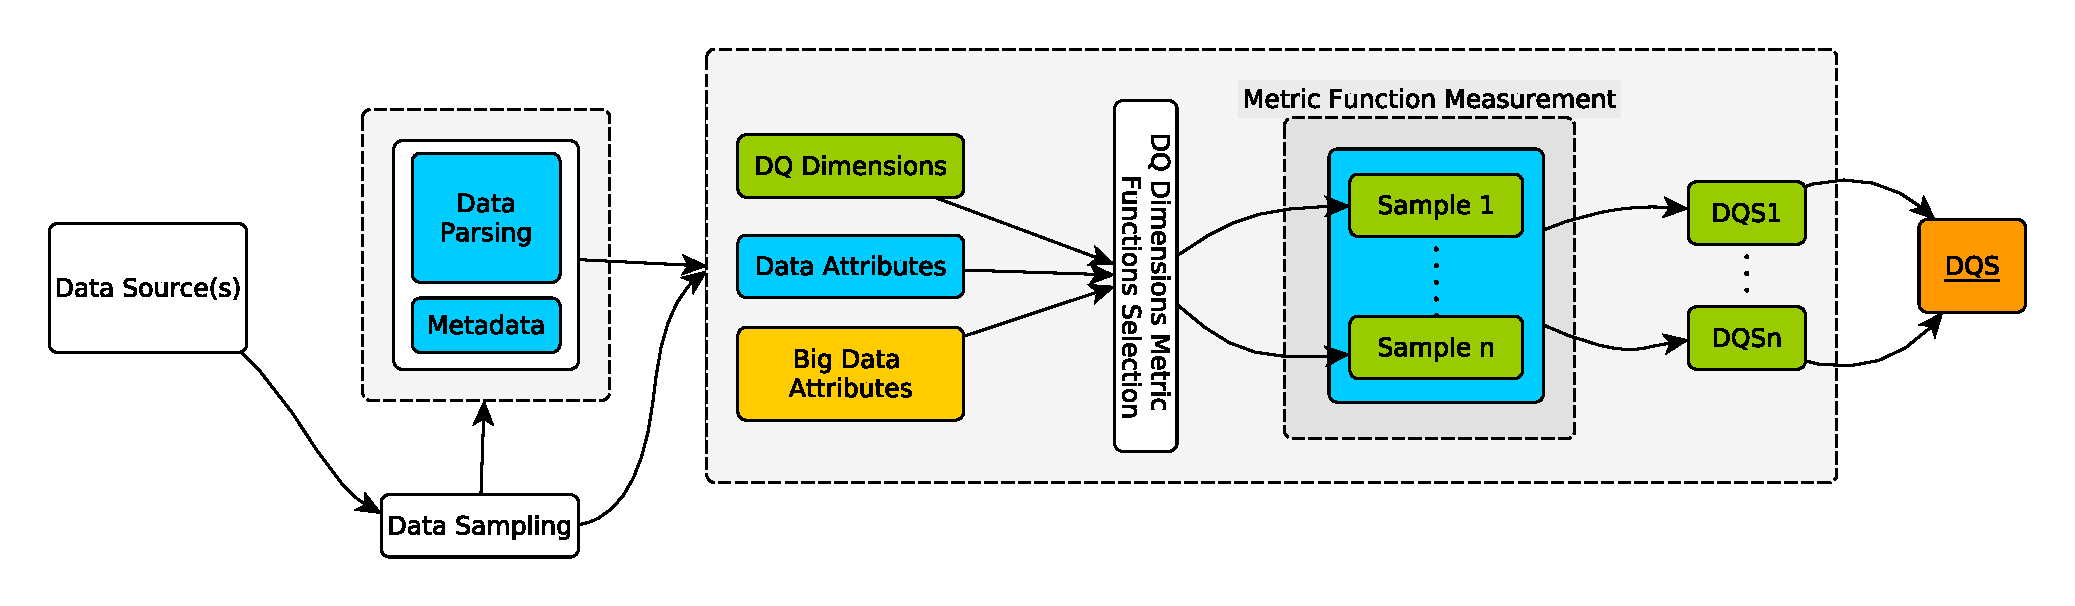
\includegraphics[scale=.55]{big_data_quality_evaluation_scheme}
	\caption{Big Data Quality Evaluation Scheme}    
\end{figure}

\section{Big Data Quality Evaluation Scheme}

The purpose of Big Data Quality Evaluation (BDQ) Scheme is to address the data quality before starting data analytics. This is done by estimating the quality of data attributes or features by applying a DQD metric to measure the quality characterized by its
accuracy, completeness or/and consistency. The expected result is data quality assessment suggestions indicating the quality 
constraints that will increase or decrease the data quality.

The BDQ Evaluation scheme is illustrated in Figure 3.1 where the data goes through many module to estimate its quality.
The key modules of our scheme consist of: (a) data sampling; and data profiling, (b) DQD vs attributes selection, 
(c) data quality Metric selection, (d) samples data quality evaluation. In the following sections, we describe each module, its input(s), output(s),
and the main functions.

\subsection{Big Data Sampling}

A sample is representative of a whole population. Based on a sample, we make several decision about a population. 
A sample is also called a subgroup. The number of observations or units in a sample is called sample size. 
The number of times a sample is collected is usually referred to as the sampling frequency. In designing a control chart, we must 
specify both of these parameters. ~\cite{Jugulum14}

There are several sampling strategies that can be applied on Big Data as expressed in ~\cite{Asilomar} ~\cite{SIGKDD}.
They evaluated the effect of sampling methods on Big Data and believed that sampling large datasets reduces run time and computational footprint of link 
prediction algorithms though maintaining sufficient prediction performance. In statistic, Bootstrap sampling technique evaluates the sampling distribution of an 
estimator by sampling with replacement from the original sample. In the context of Big Data, Bootstrap sampling has been addressed in many works 
~\cite{Liang2016} ~\cite{Satyanarayana2014}. 
In our data evaluation scheme will used the Bag of Little Bootstrap (BLB) ~\cite{ArXiv12066415}, which combines the results of bootstrapping multiple small subsets of a 
Big data dataset. THe BLB algorithm use an original Big dataset used generate small samples without replacements. 
For each generated sample another set of samples are created by resampling with replacement.

\subsection{Data Profiling}

Data profiling is an exploratory approach to data quality analysis. Statistical approaches are used to reveal 
data usage patterns as well as patterns in the data ~\cite{Osborne2013} ~\cite{Maydanchik2007}. Several tools exist for data quality assessment using data profiling 
and exploratory data analysis. Such tools include Tableau and Talend Open Studio. 

Data profiling module performs screening of data quality
based on statistics and information summary. Since
profiling is meant to discover data characteristics from data sources. It is considered as data assessment process that
provides a first summary of the data quality. Such information include: data format description, different
attributes, their types and values. data constraints (if any),
data range, max and min. More precisely information about
the data are presented in two types; technical and functional. This information can be extracted from the data itself
without any additional representation using it metadata or any descriptive header file, or by parsing the data using any
analysis tools. This task may become very costly in Big Data. To avoid costs generated due the data size we will use
the same sampling process BLB to reduce the data into a representative population sample, in addition to the combination of profiling results.

\subsection{Data Quality Evaluation}

The data profiling provides information about dataset, 

\begin{itemize}
	\item { Data attributes (eg. type format)}
	\item { Data summary (eg. max, min)}
	\item {Big data attributes; size number of sources speed of data generation (eg. data streams)}
	\item {What DQD evaluate.}
\end{itemize}

The previous information's are used to select the appropriate quality metrics functions \textbf{\textit{F}}
to evaluate a data quality dimensions \textbf{\textit{$d_k$}} for an attribute \textbf{\textit{$a_i$}}
with a weight \textbf{\textit{$w_j$}}

In the Fig 3.2 we describe how data quality evaluated using bootstrap sampling for Big data. The process
follows these steps: 

\begin{enumerate}
	\item {Sampling from the data set \textbf{S} \textbf{n} bootstrap sample size of \textbf{ss} size without replacement \textbf{$DS_j$}. }
	\item {Each sample generated from step 1 is sampled into n' samples of size SS with replacements $DS_{ij}$}
	\item {For the Each sample \textbf{$DS_{ij}$} generated in step 2, evaluate the data quality score $Q_{ij}$}	
\end{enumerate}


\begin{figure}[h]
	\vspace*{-.1in}
	\hspace*{-.6in}
	\centering
	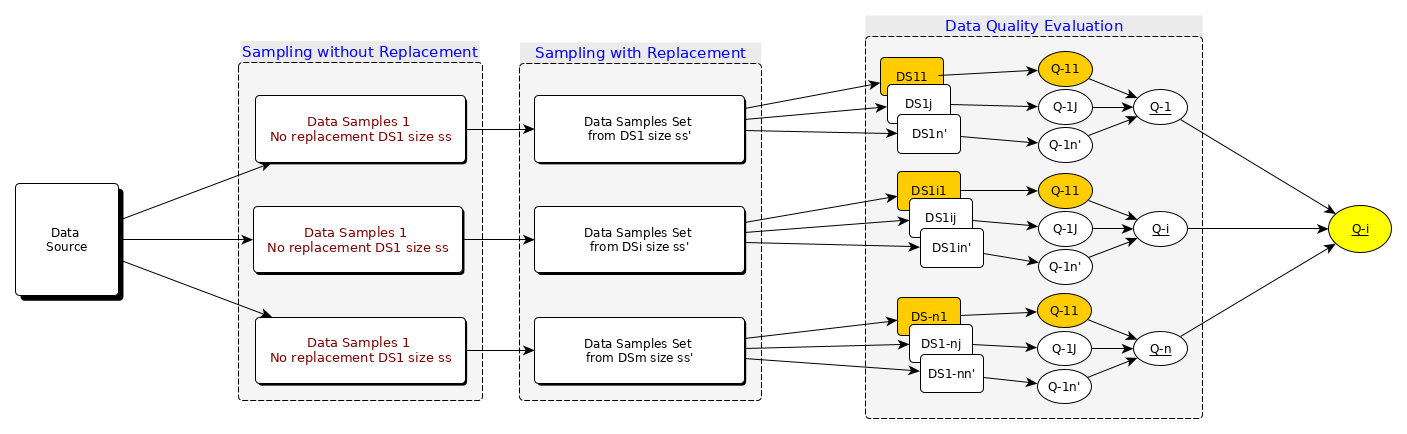
\includegraphics[scale=.38]{big-data-quality-sampling-evaluation}
	\caption{Big Data Quality Sampling Evaluation}    
\end{figure}

\begin{table}[H]
	\caption{Big Data Quality Evaluation Algorithm}
	\centering
	\begin{tabular}{p{15cm}}
	\toprule
	\textbf{Algorithm: Big Data Quality Evaluation} \\ 
	\bottomrule
	\IncMargin{1em}
	\begin{algorithm}[H]
	\SetKwData{Letds}{\textit{\textbf{let ds}}}
	\SetKwData{Letss}{\textit{\textbf{let ss}}}
	\SetKwData{Letn}{\textit{\textbf{let n}}}
	\SetKwData{Letd}{\textit{\textbf{let D}}}
	\SetKwData{Letf}{\textit{\textbf{let F}}}
	\SetKwData{Letcc}{\textit{\textbf{let cc}}}
	\SetKwData{Lets}{\textit{\textbf{let S}}}

	\SetKwData{This}{this}
	\SetKwData{Up}{up}
	\SetKwFunction{Union}{Union}
	\SetKwFunction{MetricFunctionTuple}{MetricFunctionTuple}
	
	
	\SetKwInOut{Input}{input}
	\SetKwInOut{Output}{output}
	
	\Letds a Original Data Set with size \textbf{SS and Observation (N-SS)}\; 
	\Letss  (\textbf{b(SS)}) the samples with ss < SS \;
	\Letn  samples \textbf{$s_i$} of size \textbf{ss} and \textbf{\textit{M}} Observation \textbf{(M-ss)}\;

	\Letd a set of DQD  \textbf{{$D=\{d_0,...d_k,...d_q\}$}}\;
	\Letf a metric function \textbf{F (completeness, accuracy,...)} \;
	\Letcc $\leftarrow$ 0 counter of correct valid attribute value(when \textbf{F} \textit{is true} $cc=cc+1$)\;
	\Lets \textbf{=\{ $DS_0$,...$DS_i$,...$DS_n$  \}} without replacement \;
	\BlankLine

	\For{$i\leftarrow 0$ \KwTo $n$}{
		\emph{Generate sample $s_{i}$ of size SS from ds}\;

		\For{$j\leftarrow 0$ \KwTo $n'$} {

			\emph{Generate a sample $_{ij}$ of size SS from sample $si$}\;

			\For{$k\leftarrow 0$ \KwTo $j$}{
				\MetricFunctionTuple{$d_k,F$} 
				 
				 \For{$a\leftarrow 0$ \KwTo $j$} {

				 	\For{$a_{ij}(x)$ \textbf{ss} values}{ 
						 \If{\textbf{F($a_{ij}(x)$, value) == 1}}{
							\emph{measure metric} \;
							$c\leftarrow$ cc + 1 \; 
							\emph{\textbf{Calculate the scores vector DQD(F, $d_k$,$a_{ij}$, $DS_i$})= $\frac{cc}{N}$}
							$cc\leftarrow$0 \emph{counter of correct valid attribute value \textbf{($d_k$,F)}}
						 }
					 }
					 \emph{DQD $d_k$ computed for all attributes for a sample $ds_{ij}$ }
				 }
				 \emph{$DQS_{ijk}$ is the $D_K$ scores for an attribute $a_ij$ for sample $DS_{ij}$}
				 \emph{$Q_{ijk}$ sum of all $d_k$ scores for attributes $a_{ij}$ for $DS_{ij}$ }
			}
			$Q_{ik} += 1/n'(Q_{ijk})$ 
		 }	
	}
	\emph{$Q_k$ is the mean of all $Q_{ik}$ for a specif $d_k$}
	$Q_k += 1/n(Q_{ik})$
\end{algorithm}\DecMargin{1em}
\\
\end{tabular}
\end{table}

\subsection{BDQ Evaluation Algorithm}

Let \textbf{\textit{F}} represents a set of data quality metrics, \textbf{\textit{F=\{$f_0$...$f_1$,...$f_m\}$}} 
where \textit{$f_1$} a quality metric function that will measure and evaluate a DQD \textbf{$d_k$}
for each value of an attribute $a_i$ in the sample $s_i$ and returns 1 if correct, 0 if not. 
Each $f_1$ function will compute if the value of the attribute reflects the $d_k$ constraints. 
For example, the metric accuracy of an attribute is defined as a range of values between 0 and 100,
otherwise it is correct. Similarly, it can be defined to satisfy a certain number of constraints
related to the type of data such as a zip code, email, social security number, or an address. 
If we are evaluating the same DQD $d_k$ for a set of attributes, if the weights are all equal, a simple mean 
is computed. The metric $f_i$ will be evaluated to measure if all the attributes individually 
have their $f_i$ correct. This is done for each instance (cell or row) of the sample $s_i$.

In Table 3.3, we describe the detail of BDQ Evaluation Algorithm. The $Q_k$ represents the mean
quality score for a DQD $d_k$ for measurable attributes. For data set let note. 
A as a set of attributes or features. The $Q_k$ values respectively for each attribute are represented
by a set of quality scores: 

\begin{equation*}
	V = \{Q_{ka_1},... Q_{ka_m} \}
\end{equation*}

where \textbf{A} is set of m attributes. With this evaluation, we have more insights, statistics and benefits 
about the Big data quality to ensure a well-refined analytics that targets the best precision.

\subsection{After Evaluation Analysis}

The data evaluation process done on Big data set provides
data quality information and scores of quality dimensions of
each attributes or features. These scores are used to identify
the data that must be targeted and omitted. A set of
proposals actions is generated based on many parameters,
like DQD, or data quality issue. If a data attribute got a lower score than the required level (\%) of accuracy or completeness the following actions are proposed:

\begin{itemize}
	\item{
		Discard it from the dataset.
	}
	\item {
		Tune, reformat, and normalize its values.
	}
	\item {
		Replace values, as in missing data.
	}
\end{itemize}

Whatever the Quality evaluation results, it always contains
actions to be taken on the dataset to remove any irregularities using techniques like cleaning, filtering and pre-processing based on the quality assessment.